%======================================================================
\chapter{Mechanism of \texorpdfstring{\ce{CO2}}{CO2} Reduction}\label{chap.mech}
\markright{Computational Study of the Mechanism of \texorpdfstring{\ce{CO2}}{CO2} Reduction}
%======================================================================

%======================================================================
\section{Introduction}
%======================================================================

Within two years of the appearance of the originally reported bipyridine rhenium (I) catalyst, experimental studies on the mechanism of the photocatalytic reduction of \ce{CO2} were available in the literature\autocite{kutal1985, sullivan1985}. Studies continue on the mechanism up to the present day\autocite{johnson1996, koike2002, gibson2003, hayashi2003, takeda2008, takeda2010, smieja2012, machan2014, kou2014}, utilizing new investigative techniques as they become available to elucidate transition states and transient intermediates \textit{in situ}. 

The mechanistic studies performed analyze \ce{CO2} reduction both photocatalytically and electrocatalytically on Re compounds. The electrocatalytic activity was demonstrated by Hawecker \textit{et al.} only a year after the photochemistry first appeared\autocite{hawecker1984}. Both methods involve similar cycles, and have been treated interchangeably by some authors\autocite{hayashi2003, agarwal2012b, keith2013}. The difference between electrocatalytic and photocatalytic methods is the production of the excimer species, not the reduction at the active site. Electrochemical methods have been employed with the hope of utilizing \ce{CO2} and \ce{H2O} together for the direct formation of methane and oxygen, however this problem is highly complex and the target remains elusive\autocite{roy2010, asatani2014}.

Investigation includes the use of \gls{ac.dft} methods to elucidate geometries of intermediates and transition states for the multi-step cycle. Transition metal catalysis is a non-trivial problem computationally, particularly when considering a metal from the lower period. These elements contain a large amount of electrons, many of which can be involved in non-covalent interactions with the ligands and catalyzed products. Obtaining good approximate wave functions for these complex, large systems becomes non-trivial and computationally expensive. Likely for this reason, no broad review of the mechanisms of \ce{CO2} reduction by \ce{Re^I} catalysts, investigated by \gls{ac.dft} methods, has ever been made available in the literature. 

This section will provide the first complete \gls{ac.dft} mechanistic study, from excimer formation, through key intermediates of \ce{CO2} binding and reduction, to the release of products and reformation of the catalyst. Various mechanistic pathways will be investigated, and experimental observations will be considered with the computational results. A new mechanism geometry will be proposed, tackling previously unexplained properties of the reactions.

%======================================================================
\section{Mechanism Pathways}
%======================================================================

Prior work in the literature has proposed three general mechanistic pathways for the photoreduction of \ce{CO2}\autocite{morris2009, hayashi2003, takeda2010, gibson2003}. In general, as seen in \autoref{scheme.threepath}, these pathways result in the formation of \ce{CO} and \ce{H2O}, formate (\ce{HCO2-}), or bicarbonate (\ce{HCO3-}) anions. The formation of bicarbonate proceeds via the formation of a \ce{CO2} bridged dimer that undergoes a \ce{CO2} insertion reaction to ultimately produce bicarbonate and a molecule of \ce{CO}. Production of formate requires the formation of a Re-H complex, which undergoes \ce{CO2} insertion. The formation of \ce{CO} without bicarbonate or formate by-products occurs via the coordination of \ce{CO2} to an open site on the metal, followed by a double proton addition and the release of a molecule of \ce{H2O}. This is essentially the \gls{ac.rwgsr}, wherein protons are made available from decomposition of the sacrificial amine instead of from the decomposition of \ce{H2}\autocite{kalyanasundaram1978}. These three mechanistic pathways will be referred to as the `bicarbonate' mechanism, the `formate' mechanism, and the `water-gas shift' mechanism, respectively.

\begin{scheme}[!htb]
 \begin{center}
  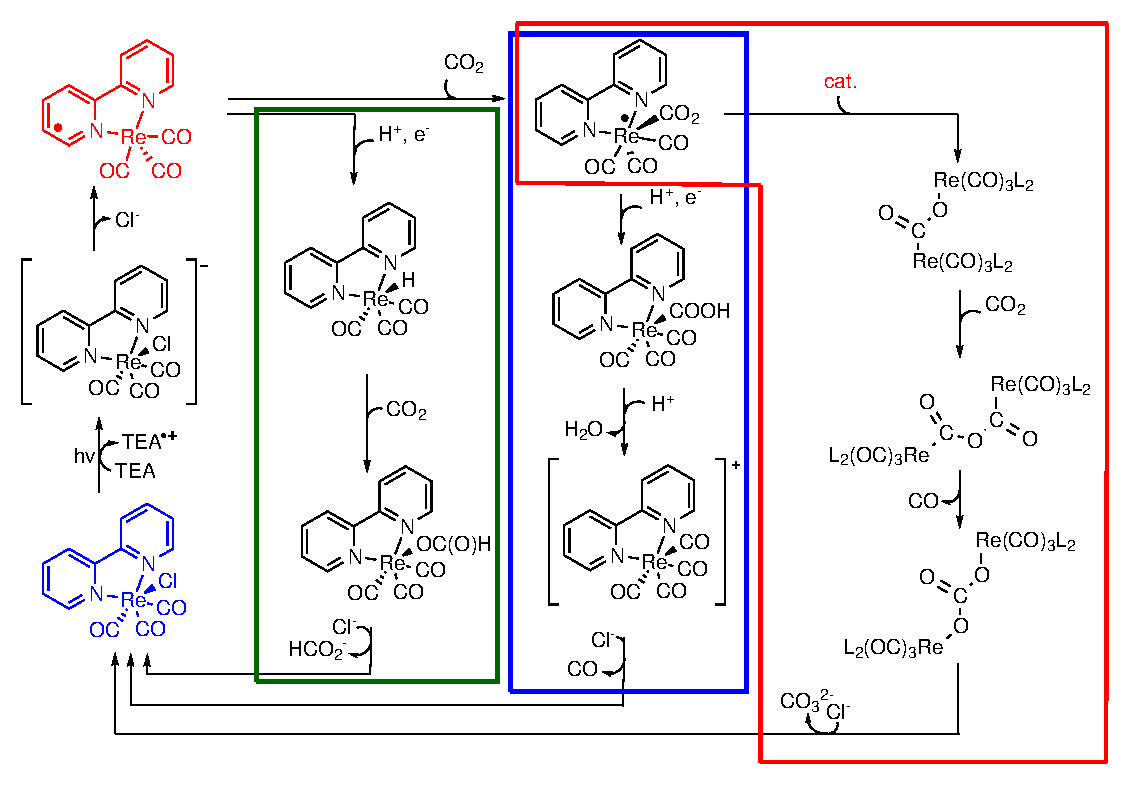
\includegraphics[clip=true, width=\textwidth, keepaspectratio]{images/threepaths.eps}
 \end{center}
\caption[Overview of mechanistic pathways.]{An overview of the mechanistic pathways of photochemical \ce{CO2} reduction. Catalyst is shown in blue, and the excimer species in red. The bicarbonate mechanism is boxed in red, the formate mechanism in green, and the water-gas shift mechanism in blue.}
\label{scheme.threepath}
\end{scheme} 

Each of the mechanistic pathways identified in \autoref{scheme.threepath} was studied, using \gls{ac.dft} methods. Structures (using 2,2'-bipyridine as the bidentate ligand, and triethylamine as the sacrificial reductant) were optimized to ground or transition states using TurboMole 6.5 software\autocite{turbomole, ahlrichs1989}, with the TPSS meta-GGA XC functional\autocite{tao2003}. This functional shows good results with organometallic complexes, while maintaining reasonable calculation times. The B3LYP functional is noted for its underestimating of transition state barriers, a complaint not levelled against TPSS\autocite{zhao2008}. The def2-TZVP all electron basis set was used for all atoms\autocite{schafer1994, weigend2005}. The TurboMole program utilizes a number of algorithms and techniques to significantly speed up the calculation times, without compromising accuracy\autocite{haase1993, treutler1995, eichkorn1997, eichkorn1995, sierka2003, deglmann2004, weigend2002, vonarnim1998, ahlrichs2004}. Grimme's dispersion correction (version 3) was included in the calculations\autocite{grimme2010}. Intermediates and transition states were verified by frequency analysis\autocite{deglmann2004, deglmann2002, grimme2002}, with further verification of transition states by performing dynamic reaction coordinate calculations to determine the \glspl{ac.irc}. The effects of solvation were calculated using the \gls{ac.cosmo} implemented in TurboMole\autocite{klamt1993}, which is a continuum solvation model implicitly surrounding the solute molecule. Code was developed to assist with automating and managing the computational jobs (see \autoref{chap.turbocontrol}).

Many of the intermediates have been synthesized in various studies \autocite{shaver1992, gibson1998, gibson1999, gibson2003}, indicating their reasonable stability. While individual portions of the mechanisms have been studied computationally in the past\autocite{agarwal2011, agarwal2012a, agarwal2012b}, no overarching study has compared methods relative to each other. Furthermore, while the formation of \ce{CO} with \ce{H2O} is the most anticipated pathway (due to the lack of formation of bicarbonate or formate in most studies), no literature pathway exists to explain the addition of \ce{CO2} to the open site of the radical catalytic species without a tri-molecular reaction step (catalyst, \ce{CO2} and \ce{H+} together) or without formate reorganization. Furthermore, no mechanism proposed thus far explains the \ce{^{12}CO} to \ce{^{13}CO} isotopic exchange demonstrated by Lehn's group in 1986\autocite{hawecker1986}. These reaction features are ignored by the studies, which prefer to focus only on the reduction of \ce{CO2}, starting from the catalyst-\ce{CO2} adducts and ending with release of \ce{CO}.

%---------------------------------------------------------------------
\subsection{Excimer Formation and Decomposition of the Sacrificial Amine}\label{ss.initiation}
%---------------------------------------------------------------------

All of the mechanistic pathways require the formation of a common excimer species, the radical 17\textit{e}\textsuperscript{-} complex (\autoref{scheme.eximer}). This occurs through the absorption of an incident photon with enough energy to promote an electron from the metal \textit{d}-orbital to the ligand $\pi^\ast$ orbitals of the ground state catalyst, \textbf{4.01}, forming the triplet \acrlong{ac.mlct} (3-MLCT) complex \textbf{\textsuperscript{3}4.01\textsuperscript{MLCT}}. This excitation requires approximately 50~kcal/mol, sourced from absorbed light. The pseudo-oxidized, electron-deficient metal atom extracts an electron from the sacrificial amine present in the reaction solution to return to the \ce{Re^{I}} state (\textbf{4.02}). However, this complex is formally a radical anion with the lone electron located in the ligand $\pi$ system, thus a halide (\textbf{4.04}) is lost to return to the neutral radical excimer species in solution, \textbf{4.03}. This electron extraction to form the radical anion catalyst and the radical cation amine is highly endothermic in the gas phase, costing over 80~kcal/mol, but in \gls{ac.dmf} it is exothermic by 5~kcal/mol. The difference in energies demonstrates the importance of performing calculations in a simulated solution; steps that may have insurmountable energy barriers in the gas phase become possible once solvation is considered.

A modestly endothermic dissociation of the chloride (15.44~kcal/mol in DMF) allows for the formation of the triplet 17~\textit{e}$^-$~excimer species \textbf{4.03}, from which the pathways discussed in following subsections may diverge.

It is important to note that some studies suggest the solvent coordinates with the excimer species \autocite{morris2009, kou2014}. This solvent coordination is expected to stabilize the excimer species in solution prior to reaction with \ce{CO2}\autocite{fujita2004}. The coordination provides approximately 11~kcal/mol of stabilization (calculated via \gls{ac.dft}). However, this event has no bearing on the overall reaction energies, as the coordination and subsequent loss of solvent is an energetically neutral occurrence and was not examined in detail.

\begin{scheme}[!htb]
 \begin{center}
  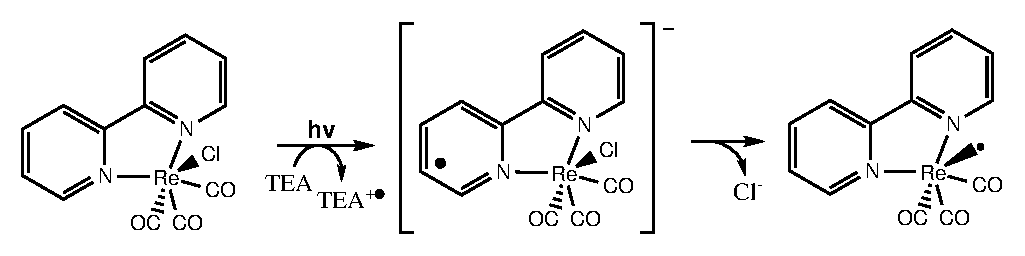
\includegraphics[clip=true, width=120mm, keepaspectratio]{images/eximer.eps}
 \end{center}
\caption[Formation of the excimer species via absorption of a photon and oxidation of the sacrificial amine.]{Formation of the excimer species via absorption of a photon and oxidation of the sacrificial amine. Energy in kcal/mol relative to the excimer \textbf{4.03} is shown in brackets for each compound.}
\label{scheme.eximer}
\end{scheme} 

The decomposition route of the sacrificial amine was first identified by Kalyansundarem in 1978\autocite{kalyanasundaram1978}, and is summarized in \autoref{scheme.decomp}. Although this work showed the decomposition of \gls{ac.teoa}, the mechanism for decomposition of \gls{ac.tea} is analogous. This decomposition is critical due to the protons it provides to the reaction mixture, and the presence of a simple second electron abstraction from the decomposition product. Upon absorption of a photon by the catalyst, the amine \textbf{4.05} is converted to the radical cationic species (\ce{Et3N+^{$\bullet$}}, \textbf{4.06}). This undergoes a proton transfer to a second molecule of the sacrificial reductant. The transfer removes a proton from the carbon $\alpha$ to the central nitrogen, leaving it a neutral radical species (forming \textbf{4.07}). This is then able to react in the catalytic cycle to provide a second electron and form the ethene-diethylamino compound \textbf{4.26}. Triethylammonium is produced as well (\textbf{4.08}), which is a proton source for the formate and water-gas shift mechanistic pathways. This step is slightly exothermic, with energy releases of 1~kcal/mol in the gas phase, and nearly 3~kcal/mol in \gls{ac.dmf}.

\begin{scheme}[!htb]
 \begin{center}
  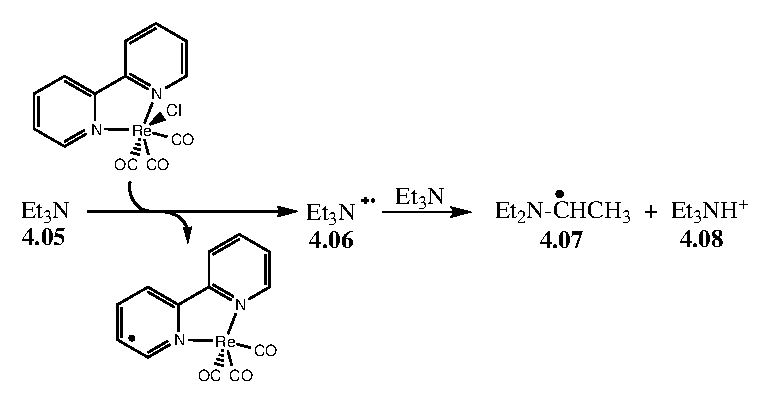
\includegraphics[clip=true, width=100mm, keepaspectratio]{images/reddecomp.eps}
 \end{center}
\caption{Decomposition pathway for the sacrificial amine.}
\label{scheme.decomp}
\end{scheme} 

Energies of each step of the reaction are listed in \autoref{tab.suprxn}. The values show a significant `uphill' series of steps requiring significant energy input. This energy is supplied by the incident photons; this process is a photocatalyzed activation. The reaction typically requires incident light of 400 nm\autocite{hawecker1983}, this high energy input allows for the excitation pathway to be followed. The potential energy diagram for these steps are shown in \autoref{fig.pes_eximer}.

% Table generated by Excel2LaTeX
\begin{table}[!htb]
\centering
 \begin{threeparttable}
  \caption{Energies for the reaction steps in the photoinduced excimer formation pathway}
    \begin{tabular}{r@{ $\rightarrow$ }lrr}
    \toprule
    \multicolumn{2}{c}{Steps} & Energy(gas)\tnote{a} & Energy(dmf)\tnote{b} \\
    \midrule
    \textbf{4.01} & \textbf{\textsuperscript{3}4.01\textsuperscript{MLCT}} & 42.81 & 53.40 \\
    \textbf{4.01\textsuperscript{3MLCT}} + \textbf{4.05} & \textbf{4.02} + \textbf{4.06} & 81.45 & -5.80 \\
    \textbf{4.02} & \textbf{4.03} + \textbf{4.04} & 50.82 & 15.44 \\
    \textbf{4.06} + \textbf{4.05} & \textbf{4.07} + \textbf{4.08} & -1.08 & -2.92 \\
    \bottomrule
    \end{tabular}%
    \begin{tablenotes}
    \item [a] TPSS energy in kcal/mol.
    \item [b] TPSS energy in kcal/mol with COSMO solvation in DMF.
    \end{tablenotes}
  \label{tab.suprxn}%
 \end{threeparttable}
\end{table}%




\begin{figure}[!htb]
 \begin{center}
  \includegraphics[clip=true, width=120mm, keepaspectratio]{images/pes_eximer.eps}
 \end{center}
\caption[Potential Energy Surface for the production of the excimer.]{Potential Energy Surface for the production of the excimer. Gas phase energies in red, DMF solvated energies in blue. A larger version can be seen in \autoref{app.energy}, \autoref{fig.apes_eximer}.}
\label{fig.pes_eximer}
\end{figure}

Some small geometry changes occur signifying the change in electron structure in the formation of the excimer species. One metric analyzed in polyaromatic non-innocent ligand redox reactions is the bonding distance between aromatic rings \autocite{bokarev2014}. From ground state to triplet MLCT complex the C-C\textsubscript{(bpy)} distance decreases from 1.47~\r{A} to 1.42~\r{A}. This 0.05~\r{A} decrease is noted in many previous experiments and calculations for anion radicals\autocite{bokarev2014, chisholm1981, castellaventura2000, gorerandall2009, irwin2010}. Other key bond lengths and angles include the ligand to metal N-Re bonds and carbonyl to metal C-Re bonds, the addition and subtraction of electrons to and from the complex impact the bond lengths. As the reaction proceeds, for example, the calculated Re-N distance in solvated structures decreases from 2.19~\r{A} in the ground state catalyst to 2.14~\r{A} in the neutral radical excimer. Similarly, the distance from the metal to the axial carbonyl decreases from 1.92 to 1.89~\r{A} in the same circumstances. Bond length changes of 0.05~\r{A} demonstrate a change has occurred in the electron configuration around the metal centre. 

%---------------------------------------------------------------------
\subsection{The `Bicarbonate' Pathway}\label{ss.carbonate}
%---------------------------------------------------------------------

The bicarbonate pathway is shown in the red box in \autoref{scheme.threepath}, with details shown in \autoref{scheme.carbonate}, starting from the excimer species. This pathway has been studied in the literature, but many details of the mechanism have not yet been explored. Previous computational analysis consists of investigation from the formed \ce{CO2} linked dimer, through the release of \ce{CO}, terminating at the carbonate linked dimer. Studies typically build the dimer as a tri-molecular step, or start with a \ce{Re\bond{-}Re} bound catalyst dimer and the insertion of \ce{CO2}\autocite{agarwal2012b}. However, the formation of the \ce{[L2Re(CO)3]2} is exceptionally slow in the presence of solvent, with a rate constant 8 orders of magnitude below the formation of the solvent-stabilized radical \ce{$^\bullet$L2Re(CO)3(solv)} complex\autocite{fujita2004}, and the \ce{[L2Re(CO)3]2} dimer is considered completely unreactive to \ce{CO2}\autocite{hayashi2003}. 

\begin{scheme}[!htb]
 \begin{center}
  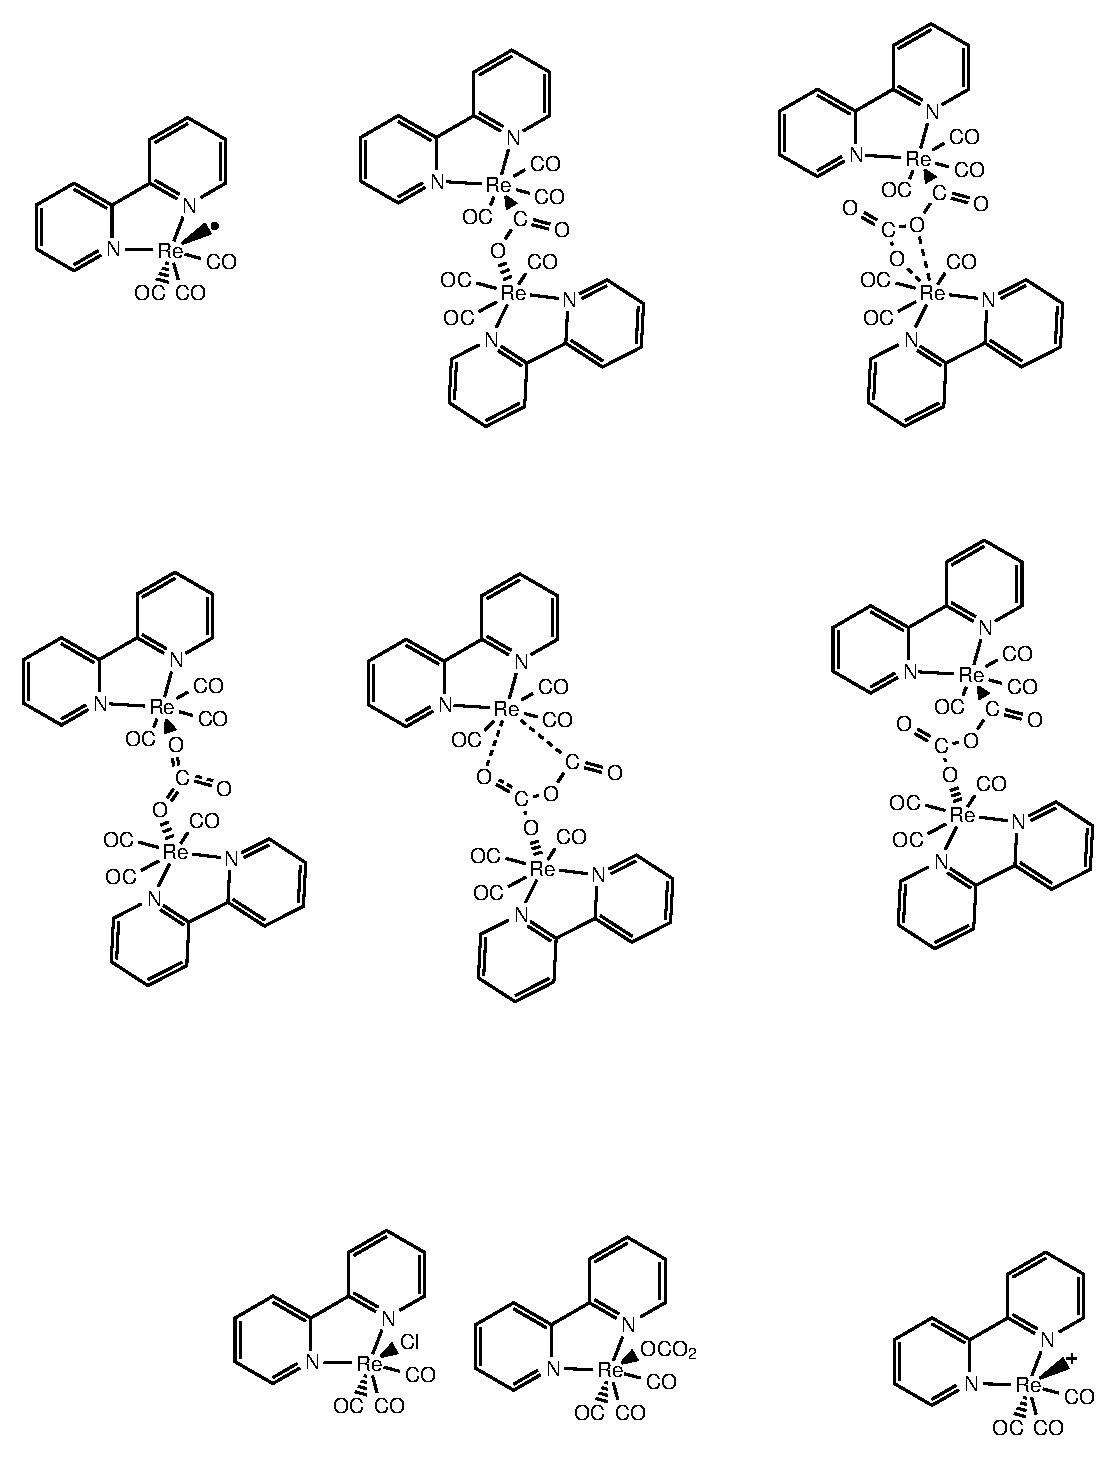
\includegraphics[clip=true, width=140mm, keepaspectratio]{images/carbonate.eps}
 \end{center}
\caption[The `bicarbonate' mechanistic pathway.]{The `bicarbonate' mechanistic pathway. Energy in kcal/mol relative to the excimer \textbf{4.03} is shown in brackets for each compound.}
\label{scheme.carbonate}
\end{scheme} 

\autoref{tab.carbrxn} shows the potential energy change in each step of the reaction. The potential energy diagram is shown in \autoref{fig.pes_carbonate} \todo{Finish making new calculated tables and figures}. The computed intermediate and transition state structures are shown in \autoref{fig.carbonatestruc}.

% Table generated by Excel2LaTeX
\begin{table}[!htb]
\centering
 \begin{threeparttable}
  \caption{Energies for the reaction steps in the `formate' pathway}
    % Table generated by Excel2LaTeX from sheet 'Tex Charts
    \begin{tabular}{rrrr}
    \toprule
    Description & Steps & Energy(gas)\tnote{a} & Energy(dmf)\tnote{b} \\
    \midrule
    Formation of Radical Anion & 4.01, 4.05 \ce{->} 4.02, 4.06   & 124.261582 & 47.596907 \\
    Open site catalyst plus cl- & 4.02 \ce{->} 4.03, 4.04 & 50.816912 & 15.440887 \\
    Reconfiguration of TEA & 4.06, 4.05 \ce{->} 4.07, 4.08 & -1.077024 & -2.915901 \\
    \midrule
    Addition of CO2 to open site & 4.4   & -0.2501423 & 6.37310903 \\
    addition of second cat to CO2 & 4.5   & 118379.026 & 118375.044 \\
    Insertion of CO2 & 4.6   & \#VALUE! & -8.5491267 \\
    relaxation of co2 insertion & 4.7   & \#VALUE! & -0.6637971 \\
    rearrange to 4ring dimer & 4.8   & \#VALUE! & \#VALUE! \\
    relax to long & 4.9   & \#VALUE! & \#VALUE! \\
    rearrangement to 5ring dimer & 4.1   & \#VALUE! & 22.4628711 \\
    relax to final & 4.11  & \#VALUE! & -24.839557 \\
    break apart & 4.12  & 317.951051 & 262.714812 \\
    return to ground states & 4.13  & -613.91666 & -426.82371 \\
    \bottomrule
    \end{tabular}%
    \begin{tablenotes}
    \item [a] TPSS SCF energy in kcal/mol.
    \item [b] TPSS SCF energy in kcal/mol with COSMO solvation in DMF.
    \end{tablenotes}
  \label{tab.carbrxn}%
 \end{threeparttable}
\end{table}%


\begin{figure}[!htb]
 \begin{center}
  \includegraphics[clip=true, width=140mm, keepaspectratio]{images/carbonatestruc.eps}
 \end{center}
\caption[DFT calculated structures for the `bicarbonate' mechanistic pathway.]{DFT calculated structures for the `bicarbonate' mechanistic pathway. Atoms are coloured as follows: carbon - grey, nitrogen - blue, oxygen - red, hydrogen - white, rhenium - teal.}
\label{fig.carbonatestruc}
\end{figure} 

\begin{figure}[!htb]
 \begin{center}
  \includegraphics[clip=true, width=140mm, keepaspectratio]{images/pes_carbonate.eps}
 \end{center}
\caption[Potential Energy Surface for the bicarbonate mechanistic pathway.]{Potential Energy Surface for the bicarbonate mechanistic pathway. Gas phase energies in red, DMF solvated energies in blue. A larger version is available in \autoref{app.energy}, \autoref{fig.apes_carbonate}.}
\label{fig.pes_carbonate}
\end{figure}

The mechanism begins with the addition of a \ce{CO2} molecule to the excimer \textbf{4.03}, forming \textbf{4.11}. This is a very weakly bound species when solved in a simulated \gls{ac.dmf} environment; in the gas phase this transition complex will not solve. Energies for the gas phase for this compound are calculated as single point energies from the solvated structure. The \gls{ac.dmf} solved structure has a Re-C bond length of 2.51~\r{A}, and O-C-O bonding angle of 142$^\circ$, when compared to the \ce{Re\bond{-}C} distances of rhenium carbonyls of \textit{ca.} 1.9~\r{A}, this is a very weak bond. The formation of this complex requires only 6.37~kcal/mol, the electron is unpaired in this new structure as well. An additional electron is required to form a more stable compound. This unstable complex is able to extract a hydrogen from triethylammonia (\ce{Et3NH+}, \textbf{4.08}) to continue with the `water-gas' pathway (see below \autoref{ss.watergas}), or combine with a second molecule of the excimer to form a dimer \textbf{4.12}. This dimer formation is exothermic by 42.4~kcal/mol in \gls{ac.dmf}. The quenching of the radical forms much stronger bonds between the metal atoms and the linking \ce{CO2}. The Re-C distance has shortened from the 2.51~\r{A} seen in \textbf{4.11} to 2.26~\r{A}. This is still longer than the Re-CO bonds, which is expected due to the lack of $\pi$ back-bonding observed with carbonyl ligands, however, it corresponds with similar published crystal structures of Re-C bond lengths for sp\textsuperscript{2} carbons\autocite{lukehart1977}. The Re-O bond is 2.13~\r{A}, a value that remains constant for Re-O through the intermediates in the reaction pathway.

After the dimer \textbf{4.12} has been formed, a second molecule of \ce{CO2} is inserted via transition state \textbf{4.13} to form the Re-C(O)-O-C(O)-O-Re complex \textbf{4.14}. This \ce{C2O4} linker contains \ce{C\bond{-}O} single bonds of length 1.28~\r{A}, and \ce{C\bond{=}O} double bonds of 1.44~\r{A}, longer than expected by about 0.1~\r{A} for both sp\textsuperscript{2} carbon-oxygen single or double bonds \autocite{crc1998}. Bond angles are typically just under the idealized 120$^\circ$ expected as well. Due to the linker, the two catalyst ligand bipyridines have moved from a nearly co-planar geometry to a nearly perpendicular geometry. Re-C and Re-O bonds remain constant in length compared to \textbf{4.12}. The formation of a 5 membered ring transition state structure \textbf{4.15} costs 22~kcal/mol. This leads to the release of the \ce{CO} and the formation of a carbonate linked dimer, \textbf{4.16}, resulting in a net energy decrease of -2.4~kcal/mol, and returning the catalyst ligands to a more co-planar orientation. The carbonate dimer species is left to decompose to a catalyst cation \textbf{4.19} with an open site, and the carbonate adduct \textbf{4.17}. This carbonate dianion may pick up a proton before or after the disassociation to the catalyst cationic species, resulting in the released of the bicarbonate species to solution (\textbf{4.18)} when the catalyst is returned to ground state \textbf{4.01} with addition of a chloride. The decomposition of the bicarbonate dimer species is very endothermic, by 262~kcal/mol in \gls{ac.dmf}. This is due to the charge separations that occur, while \gls{ac.cosmo} solvation stabilizes these charged species, it does not accurately simulate a system with an ionic strength similar to what could be expected in the experimental reaction. The Gibbs energy for this step was calculated to be -11.4~kcal/mol in solution, with an additional -17~kcal/mol for the anion exchange, signifying the thermodynamic favourableness of this transformation. The presence of excess molar equivalents of an electrolyte such as tetraethylammoniumchloride ensures a surplus of chloride anions are in solution and are an additional force for conversion, according to Le Ch\^{a}telier's principle.

%---------------------------------------------------------------------
\subsection{The `Formate' Pathway}\label{ss.formate}
%---------------------------------------------------------------------
In comparison to the catalytic dimer formed in the bicarbonate pathway above, the formate formation occurs via a much simpler mechanism. This mechanism is shown in the green box in \autoref{scheme.threepath}, with details shown in \autoref{scheme.formate}. The addition of a hydrogen to the open site axial to the metal occurs via the simultaneous electron and proton transfer from a by-product of the reduction of the amine. \ce{CO2} inserts into this metal hydride bond, resulting in the formate ligand bonded through the oxygen center\autocite{sullivan1984, sullivan1986, creutz2007}. Separation of the weak metal-oxygen bond allows for the substitution of the halide to the cationic metal centre. 

\begin{scheme}[!htb]
 \begin{center}
  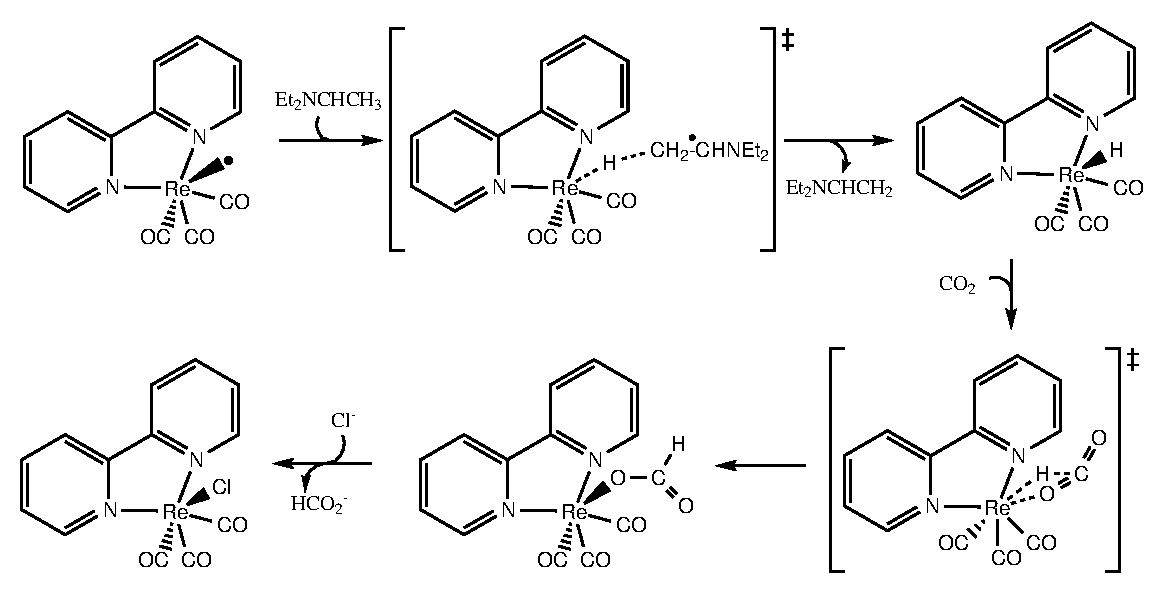
\includegraphics[clip=true, width=\textwidth, keepaspectratio]{images/formate.eps}
 \end{center}
\caption[The `formate' mechanistic pathway.]{The `formate' mechanistic pathway. Energy in kcal/mol relative to the excimer \textbf{4.03} is shown in brackets for each compound.}
\label{scheme.formate}
\end{scheme} 

\autoref{tab.formrxn} shows the potential energy change in each step of the reaction. The computed intermediate and transition state structures are shown in \autoref{fig.formatestruc}.

% Table generated by Excel2LaTeX
\begin{table}[!htb]
\centering
 \begin{threeparttable}
  \caption{Energies for the reaction steps in the `formate' pathway}
    % Table generated by Excel2LaTeX from sheet 'Tex Charts
    \begin{tabular}{rrrr}
    \toprule
    Description & Steps & Energy(gas)\tnote{a} & Energy(dmf)\tnote{b} \\
    \midrule
    Formation of Radical Anion & 1.1   & -39.271301 & -67.827267 \\
    Open site catalyst plus cl- & 1.2   & 50.8169125 & 15.4408871 \\
    Reconfiguration of TEA & 1.3   & -164.60991 & -118.34007 \\
    \midrule
    Hydride Extraction & 1.4   & 4.09794743 & -9.8319638 \\
    Removal of TEA & 1.5   & -26.652434 & -20.021496 \\
    Insertion of CO2 & 1.6   & 21.2356096 & 14.0177223 \\
    recoordination & 1.7   & -33.936535 & -28.657394 \\
    dissasotiation of HCO2- & 1.8   & 140.389052 & 39.6680755 \\
    Reformation of Catalyst & 1.9   & -141.76995 & -36.367745 \\
    \bottomrule
    \end{tabular}%
    \begin{tablenotes}
    \item [a] TPSS SCF energy in kcal/mol.
    \item [b] TPSS SCF energy in kcal/mol with COSMO solvation in DMF.
    \end{tablenotes}
  \label{tab.formrxn}%
 \end{threeparttable}
\end{table}%



\begin{figure}[!htb]
 \begin{center}
  \includegraphics[clip=true, width=140mm, keepaspectratio]{images/formatestruc.eps}
 \end{center}
\caption[DFT calculated structures for the `formate' mechanistic pathway.]{DFT calculated structures for the `formate' mechanistic pathway. Atoms are coloured as follows: carbon - grey, nitrogen - blue, oxygen - red, hydrogen - white, rhenium - teal.}
\label{fig.formatestruc}
\end{figure} 

\begin{figure}[!htb]
 \begin{center}
  
\includegraphics[clip=true, width=140mm, keepaspectratio]{images/pes_formate.eps}
 \end{center}
\caption[Potential Energy Surface for the formate mechanistic pathway.]{Potential Energy Surface for the formate mechanistic pathway. Gas phase energies in red, DMF solvated energies in blue. A larger version can be seen in \autoref{app.energy}, \autoref{fig.apes_formate}.}
\label{fig.pes_formate}
\end{figure} 

After formation of the excimer \textbf{4.03}, the radical species extracts a hydrogen atom from the oxidized chain of the sacrificial amine \textbf{4.07} in transition state \textbf{4.21}, a step endothermic by 21.0~kcal/mol in the gas phase and 20.9~kcal/mol in \gls{ac.dmf}. The radical amine (\textbf{4.07}) had been previously formed (see \autoref{ss.initiation}). Extraction of the proton and electron pair allows for the formation of the ethene, completing the decomposition of the amine to the final neutral, singlet molecule \textbf{4.26}. Relaxation of this transition state results in the hydrogen extraction from the radical species, yielding the formation of the hydride complex \textbf{4.22}, a step exothermic by 50.7~kcal/mol in DMF.

This hydride complex is able to insert a molecule of \ce{CO2} into the metal-hydrogen bond, in transition step \textbf{4.23}, with a 14.4~kcal/mol barrier to transition state formation. \ce{CO2} insertion to metal hydrides is commonly observed, most mechanisms in \ce{CO2} reduction in similar ruthenium systems employ this addition\autocite{creutz2007}. The Re-H bond length is 1.76~\r{A}, compared to the length of the Re-Cl bond from the ground state \textbf{4.01} species of 2.51~\r{A}. This bond length difference reflects the observations on anion change from Cl to Br (as discussed in \autoref{chap.newchem}, \autoref{ss.xray}), the anion size is the critical factor in this variation. When a molecule of \ce{CO2} approaches, the transition state of a pseudo-septacoordinate species \textbf{4.23} forms. The Re-H bond increases in length to 2.16~\r{A}, the Re-O bond is 2.88~\r{A}, and the O-Re-H angle is very tight, at only 45.3$^\circ$. This step completes with 28.66~kcal/mol energy release to form the formato anion complex \textbf{4.24}. 

The formato anion \textbf{4.24} contains a Re-O bond of 2.15~\r{A}, consistent with previously discussed rhenium - oxygen bonds. This formate dissociates with a chloride addition, the exchange is endothermic by less than 3~kcal/mol overall, but the charge separated transition state formation is endothermic by nearly 40~kcal/mol in DMF (or 140~kcal/mol in gas phase). As discussed with the bicarbonate mechanism, this large cost is due to the charge separation that occurs. The calculated Gibbs energy for the formation of the charge separated transition state is -12.7~kcal/mol in solvent, showing the thermodynamic favourableness of this exchange. Further reactions of the formato anion in solution are not investigated, but the anion may remain deprotonated in the slightly basic environment\autocite{morimoto2013}. 

It is possible that the mechanistic cycle restarts with \textbf{4.24} absorbing a photon instead of substituting for the chloride. This would not affect the next catalytic cycle; either anion is lost in formation of the excimer.

Some attempts were made at performing the \ce{CO2} binding reaction by alternative geometries. While direct $\sigma$ bonding from a metal to an oxygen atom in the \ce{CO2} molecule (as $\eta^1$-OCO) has been observed in a few systems (including photoreduction of \ce{CO2} on other metal systems)\autocite{lee2001, mauser2001, souter1997}, this geometry is rare\autocite{castrorodriguez2004, cokoja2011, gibson1996}. Attempts to coordinate \ce{CO2} in an $\eta^1$-OCO geometry failed to converge both in gas and solution phase, as \ce{CO2} was ejected from the complex. Binding of \ce{CO2} to the metal through $\pi$ coordination of the C=O bond is more common\autocite{cokoja2011, gibson1996}, but these structures failed to solve in the current \gls{ac.dft} system as well.

\FloatBarrier

%---------------------------------------------------------------------
\subsection{The `Water-Gas Shift' Pathway}\label{ss.watergas}
%---------------------------------------------------------------------
The water-gas shift mechanism involves the addition of two protons from the reductant to a \ce{CO2} molecule bound to the metal centre, as shown in the blue box in \autoref{scheme.threepath}. The mechanism is shown in greater detail in \autoref{scheme.watergas}. The first proton addition yields an acid species, this is dehydrated via the second addition of a proton and the release of one molecule of \ce{H2O}. The resulting tetracarbonyl cationic species is able then to release an axial carbonyl to return to the ground state. While any of the carbonyl groups could be labile, either of the carbonyl ligands at the axial positions are the ones actively replaced by the halide to return to the starting catalyst\autocite{shaver1992}. 

\begin{scheme}[!htb]
 \begin{center}
  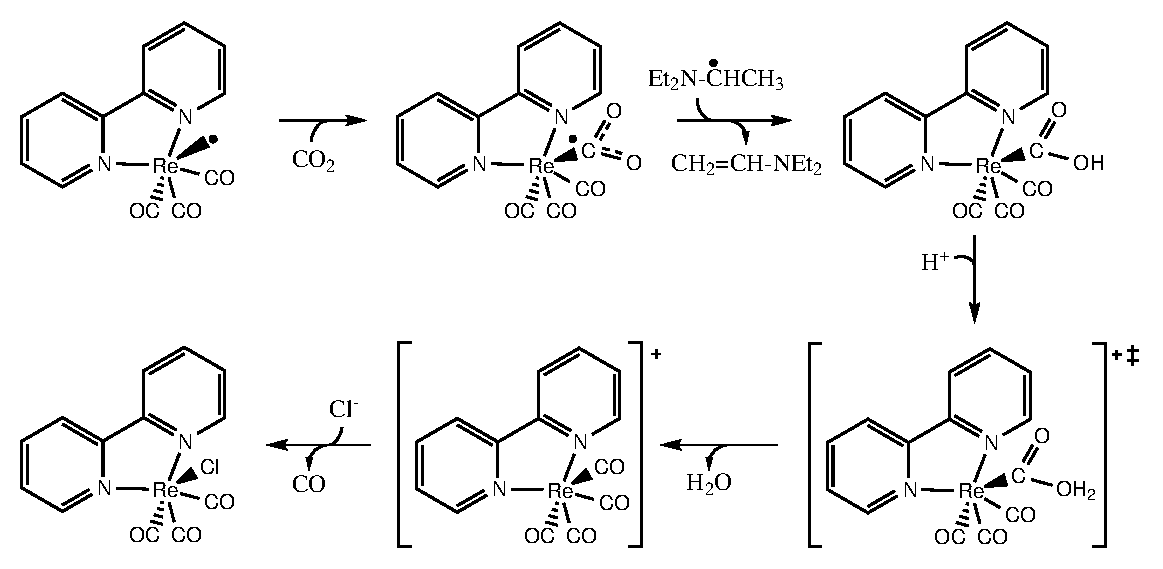
\includegraphics[clip=true, width=\textwidth, keepaspectratio]{images/watergas.eps}
 \end{center}
\caption[The `water-gas shift' mechanistic pathway.]{The `water-gas shift' mechanistic pathway. Energy in kcal/mol relative to the excimer \textbf{4.03} is shown in brackets for each compound.}
\label{scheme.watergas}
\end{scheme} 

\autoref{tab.wgsrxn} shows the potential energy change in each step of the reaction. The potential energy surface is shown in \autoref{fig.pes_axial}. The computed intermediate and transition state structures are shown in \autoref{fig.wgsaxstruc}.

% Table generated by Excel2LaTeX
\begin{table}[!htb]
\centering
 \begin{threeparttable}
  \caption{Energies for the reaction steps in the `formate' pathway}
    \begin{tabular}{rrrr}
    \toprule
    Description & Steps & Energy(gas)\tnote{a} & Energy(dmf)\tnote{b} \\
    \midrule
    Formation of Radical Anion & 2.1   & -39.271301 & -67.827267 \\
    Open site catalyst plus cl- & 2.2   & 50.8169125 & 15.4408871 \\
    Reconfiguration of TEA & 2.3   & -164.60991 & -118.34007 \\
    \midrule
    migration of open site? & 2.4   & 23.3674263 & 19.7662463 \\
    Addition of CO2 to open site & 2.5   & 4.78987184 & 1.56207334 \\
    H transfer to CO2 & 2.6   & -61.998066 & -35.596525 \\
    CO2H planar relaxation & 2.7   & 22.2489536 & -5.1943905 \\
    COOH2 ts & 2.8   & 144.908364 & 116.570584 \\
    CO4 + and water & 2.9   & 4.10436095 & -1.4970678 \\
    dissassotiation of CO & 2.10  & 40.893777 & 35.5673996 \\
    Reformation of Catalyst & 2.11  & -141.76995 & -36.367745 \\
    \bottomrule
    \end{tabular}%
    \begin{tablenotes}
    \item [a] TPSS SCF energy in kcal/mol.
    \item [b] TPSS SCF energy in kcal/mol with COSMO solvation in DMF.
    \end{tablenotes}
  \label{tab.wgsrxn}%
 \end{threeparttable}
\end{table}%




\begin{figure}[!htb]
 \begin{center}
  \includegraphics[clip=true, width=100mm, keepaspectratio]{images/wgsaxialstruc.eps}
 \end{center}
\caption[DFT calculated structures for the axial `water-gas shift' mechanistic pathway.]{DFT calculated structures for the axial `water-gas shift' mechanistic pathway. Atoms are coloured as follows: carbon - grey, nitrogen - blue, oxygen - red, hydrogen - white, rhenium - teal.}
\label{fig.wgsaxstruc}
\end{figure}

\begin{figure}[!htb]
 \begin{center}
  \includegraphics[clip=true, width=140mm, keepaspectratio]{images/pes_axial.eps}
 \end{center}
\caption[Potential Energy Surface for the axial geometry of the water-gas shift mechanistic pathway.]{Potential Energy Surface for the axial geometry of the water-gas shift mechanistic pathway. Gas phase energies in red, DMF solvated energies in blue. A larger version can be seein in \autoref{app.energy}, \autoref{fig.apes_axial}.}
\label{fig.pes_axial}
\end{figure} 

This mechanistic pathway appears to begin by the same addition of \ce{CO2} that is seen in the bicarbonate mechanism (see \autoref{ss.carbonate}), forming \textbf{4.11}. As before, the complex is only weakly coordinated, and requires solvation effects to solve computationally. The added \ce{CO2} is able to extract a hydrogen from the previously-reduced sacrificial amine \textbf{4.07} with a net energy change of -35.1~kcal/mol in \gls{ac.dmf}, again allowing the formation of the ethene amine \textbf{4.26}. The newly formed acid species \textbf{4.32} dehydrates in the presence of a second proton (via \textbf{4.33}) to form water \textbf{4.37} and the tetracarbonyl cationic species \textbf{4.38}. This is endothermic by 8.9~kcal/mol in solution, but the $\Delta$G is -15~kcal/mol. This tetracarbonyl cation exchanges a \ce{CO} molecule for a \ce{Cl-} to return to \textbf{4.01}, with a 0.8~kcal/mol energy release. 

Typically, this reaction had been thought to proceed on the axial site of the catalyst, mirroring the pathways discussed above. However, due to the ease of migration of carbonyl groups in organometallic complexes, it is proposed that the `water-gas shift' mechanism does not occur axial to the ligand, but begins with relocation of a \ce{CO2} ligand to the axial position (see \autoref{scheme.rearrange}), followed by the coordination of \ce{CO2} into the now vacant planar open site, forming \textbf{4.35}. Potential energies for this reaction are shown in \autoref{tab.siderxn}, and the potential energy diagram is shown in \autoref{fig.pes_planar}. \Gls{ac.dft} computed structures are shown in \autoref{fig.wgseqstruc}. 

\begin{scheme}[!htb]
 \begin{center}
  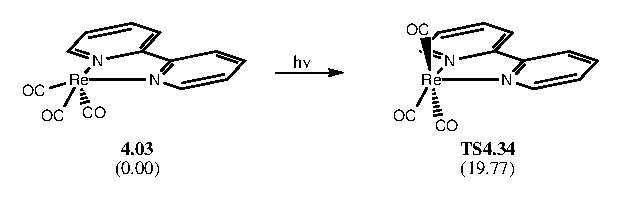
\includegraphics[clip=true, width=120mm, keepaspectratio]{images/rearrange.eps}
 \end{center}
\caption[Rearrangement of carbonyl and open site.]{Rearrangement of carbonyl and open site. Energy in kcal/mol relative to the excimer \textbf{4.03} is shown in brackets for each compound.}
\label{scheme.rearrange}
\end{scheme}

% Table generated by Excel2LaTeX
\begin{table}[!htb]
\centering
 \begin{threeparttable}
  \caption{Energies for the reaction steps in the `formate' pathway}
    % Table generated by Excel2LaTeX from sheet 'Tex Charts
    \begin{tabular}{rrrr}
    \toprule
    Description & Steps & Energy(gas)\tnote{a} & Energy(dmf)\tnote{b} \\
    \midrule
    Formation of Radical Anion & 4.01, 4.05 \ce{->} 4.02, 4.06   & 124.261582 & 47.596907 \\
    Open site catalyst plus cl- & 4.02 \ce{->} 4.03, 4.04 & 50.816912 & 15.440887 \\
    Reconfiguration of TEA & 4.06, 4.05 \ce{->} 4.07, 4.08 & -1.077024 & -2.915901 \\
    \midrule
    Addition of CO2 to open site & 3.4   & -0.2501423 & 6.37310903 \\
    H transfer to CO2 & 3.5   & -19.133571 & -33.878805 \\
    CO2H axial relaxation & 3.6   & -0.2145456 & -1.1883574 \\
    COOH2 ts & 3.7   & 151.907871 & 125.579781 \\
    CO4 + and water & 3.8   & 5.1112987 & -1.2748062 \\
    dissassotiation of CO & 3.9   & 40.893777 & 35.5673996 \\
    Reformation of Catalyst & 3.10  & -141.76995 & -36.367745 \\
    \bottomrule
    \end{tabular}%
    \begin{tablenotes}
    \item [a] TPSS SCF energy in kcal/mol.
    \item [b] TPSS SCF energy in kcal/mol with COSMO solvation in DMF.
    \end{tablenotes}
  \label{tab.siderxn}%
 \end{threeparttable}
\end{table}%




\begin{figure}[!htb]
 \begin{center}
  \includegraphics[clip=true, width=140mm, keepaspectratio]{images/wgseqstruc.eps}
 \end{center}
\caption[DFT calculated structures for the equatorial `water-gas shift' mechanistic pathway.]{DFT calculated structures for the equatorial `water-gas shift' mechanistic pathway. Atoms are coloured as follows: carbon - grey, nitrogen - blue, oxygen - red, hydrogen - white, rhenium - teal.}
\label{fig.wgseqstruc}
\end{figure} 

\begin{figure}[!htb]
 \begin{center}
  \includegraphics[clip=true, width=140mm, keepaspectratio]{images/pes_planar.eps}
 \end{center}
\caption[Potential Energy Surface for the planar geometry of the water-gas shift mechanistic pathway.]{Potential Energy Surface for the planar geometry of the water-gas shift mechanistic pathway. Gas phase energies in red, DMF solvated energies in blue. A larger version can be seen in \autoref{app.energy}, \autoref{fig.apes_planar}.}
\label{fig.pes_planar}
\end{figure} 

This \ce{CO2} bound in the plane of the ligand then undergoes hydrogen addition and dehydration to produce a molecule of \ce{H2O}, continuing as before. Once reduced to the tetracarbonyl cluster, the catalyst could shed any \ce{CO} ligand and pick up a chloride anion to return to the neutral ground state. However, labilization of one of the two axial carbonyls is the most favoured, formation of the planar coordinated chloride complex is not expected\autocite{shaver1992}.

This newly proposed mechanism provides an explanation to a previously unexplained phenomenon. The exchange of carbonyl groups on the catalyst for \ce{^{13}CO} when using \ce{^{13}CO2} in the photoreduction is documented as early as Hawecker \textit{et al.} in 1986\autocite{hawecker1986}. It was shown that complete exchange occurs with very few catalytic turnovers. Furthermore, Koike \textit{et al.} demonstrated that photochemical ligand substitution occurs at only axial sites relative to the $\alpha$-imino ligand\autocite{koike2002}, no exchange occurs at the equatorial site, nor can the \textit{fac}-\ce{(^{12}CO)2^{13}CO} be expected to shift the \ce{^{13}CO} to the equatorial position in the time-frame of the reaction. Thus the isotopic exchange does not proceed by independent uptake of produced \ce{^{13}CO}, instead the conversion to the \ce{^{13}CO} complex must be inherent in the reduction mechanism. 

This modified geometry does not violate any previously published experimental mechanism work. These studies typically focus on photophysical or spectroscopic analysis to determine intermediates. The analysis methods used define molecular composition; they are not structural characterization techniques. Re-evaluation of the spectral data within these newly defined parameters does not invalidate the work, mechanistic descriptors published (such as kinetics) are still valid within the new geometry.

Additionally, this provides an explanation for the lack of \ce{CO2} reduction by (terpy)-$\kappa^2$-\ce{Re(CO)3Cl} discussed in \autoref{chap.co2}. While the carbonyl group is transitioning to the axial site, before a molecule of \ce{CO2} has been coordinated to the complex, the catalyst is in optimal geometry for chelation of the pendant arm (see \autoref{scheme.tricarbonyl}) as discussed in \autoref{chap.co2}. It was previously shown that the tridentate catalyst is inactive for \ce{CO2} photoreduction, the formation of a $\kappa^3$ complex modifies the photophysics, deactivating the catalyst's reactivity.

\FloatBarrier

%======================================================================
\section{Comparison Between Mechanistic Pathways} \label{sec.compare}
%======================================================================

Previous studies in literature had only analyzed one of the mechanistic pathways (or a subset), without a fuller analysis of the competitiveness of each pathway relative to the others. Discussion on the tenability of each potential pathway relied on the \textit{in situ} observation of intermediates or transition states, the success (or lack thereof) of synthesis of the intermediates, and the relative production of by-products in the mechanistic trials. 

The overall potential energy diagrams for each of the mechanistic pathways given in \autoref{scheme.threepath} are shown in \autoref{fig.threeenergies}. Individual mechanistic pathways, and separate potential energy diagrams for gas phase and \gls{ac.dmf} solvated structures are listed in \autoref{app.energy}. This figure shows the difficulty in determining the most likely reaction pathway based on computational analysis alone. The difference in energy consumption between mechanisms is quite small, with the largest barriers belonging to the final disassociation of the product and coordination of chloride.

\begin{figure}[!htb]
 \begin{center}
  \includegraphics[clip=true, width=140mm, keepaspectratio]{images/pes_dmf.eps}
 \end{center}
\caption[An overview of the energies of the three mechanistic pathways of photochemical \ce{CO2} reduction in DMF.]{An overview of the energies of the three mechanistic pathways of photochemical \ce{CO2} reduction in DMF. Excimer formation is shown in blue, the planar water-gas shift mechanism in red, the axial water-gas shift in orange, the bicarbonate in purple, and the formate in green.}
\label{fig.threeenergies}
\end{figure}  

Experimental data shows that each of the mechanisms is feasible and could occur in certain conditions. Both the formate and water-gas routes have the maximum transition energy barrier for the final disassociation of the product and coordination of chloride. This barrier is artificially high, the charge separation that occurs is impacted significantly by the basic pH and the presence of electrolyte in solution experimentally. These factors are not taken into consideration in the calculations. Gibbs energies were calculated for these steps, the average $\Delta$G values are around -12~kcal/mol for the production of the transition state, signifying a thermodynamically favoured reaction. 

Due to the similarity in potential energy profiles for these reactions, analysis of experimental data must be undertaken to accurately predict which pathway dominates the photoreduction of \ce{CO2}. The energy requirements of each pathway is not the only indicator of mechanistic preference. Studies have shown the rate differs between pathways, with the formation of certain intermediates being so slow as to nearly block the progression of the redox reaction. Utilization of modified reaction conditions (\gls{ac.tea} vs. \gls{ac.teoa}, changing solvent mixture, presence or absence of \ce{H2O}, presence or absence or modification of electrolyte) can provide a range of reduction products, by-products, and intermediates\autocite{hawecker1983, hawecker1986, sullivan1985, hayashi2003, morris2009, morimoto2013}.

%======================================================================
\section{Conclusions} 
%======================================================================

Three feasible mechanistic pathways for the photocatalytic reduction of \ce{CO2} were investigated in detail using consistent \gls{ac.dft} methods, allowing for their comparison. Mechanistic steps not previously elucidated were demonstrated, showing the full mechanistic cycle from ground state excitation through the reaction of the excimer with \ce{CO2} to the final release of product and reforming of catalyst. 

A modified geometry for the production of \ce{CO} and \ce{H2O} by the `water-gas' mechanism was proposed. This new geometry does not conflict with previously published experimental data, and provides explanation for previously reported phenomenon. It aligns with the previously demonstrated inactivity of terpyridine catalysts, in contrast to the highly active bipyridine analogue. This new geometry provides an avenue for the isotopic exchange of carbonyl ligands from \ce{^{12}CO} to \ce{^{13}CO} when the reduction is carried out with \ce{^{13}CO2}. 
